\subsection{Gaseous species}\label{sec:gas}
Fig.~\ref{fig:thx_ch4}a-c presents the time-histories of CH$_4$ mole fraction at two representative conditions, T$_5$$\approx1900$~K and 2200~K, for 5\%, 10\%, and 30\% CH$_4$. Absorption cross-sections ($\sigma_v$) were calculated using simulated temperatures with FFCM2 and shown in Fig.~\ref{fig:ch4absfit}.
Overall, model predictions agree more closely with measurements at 5\% and 10\% CH$_4$ than at 30\% CH$_4$.

\begin{figure}[!t]
	\centering
	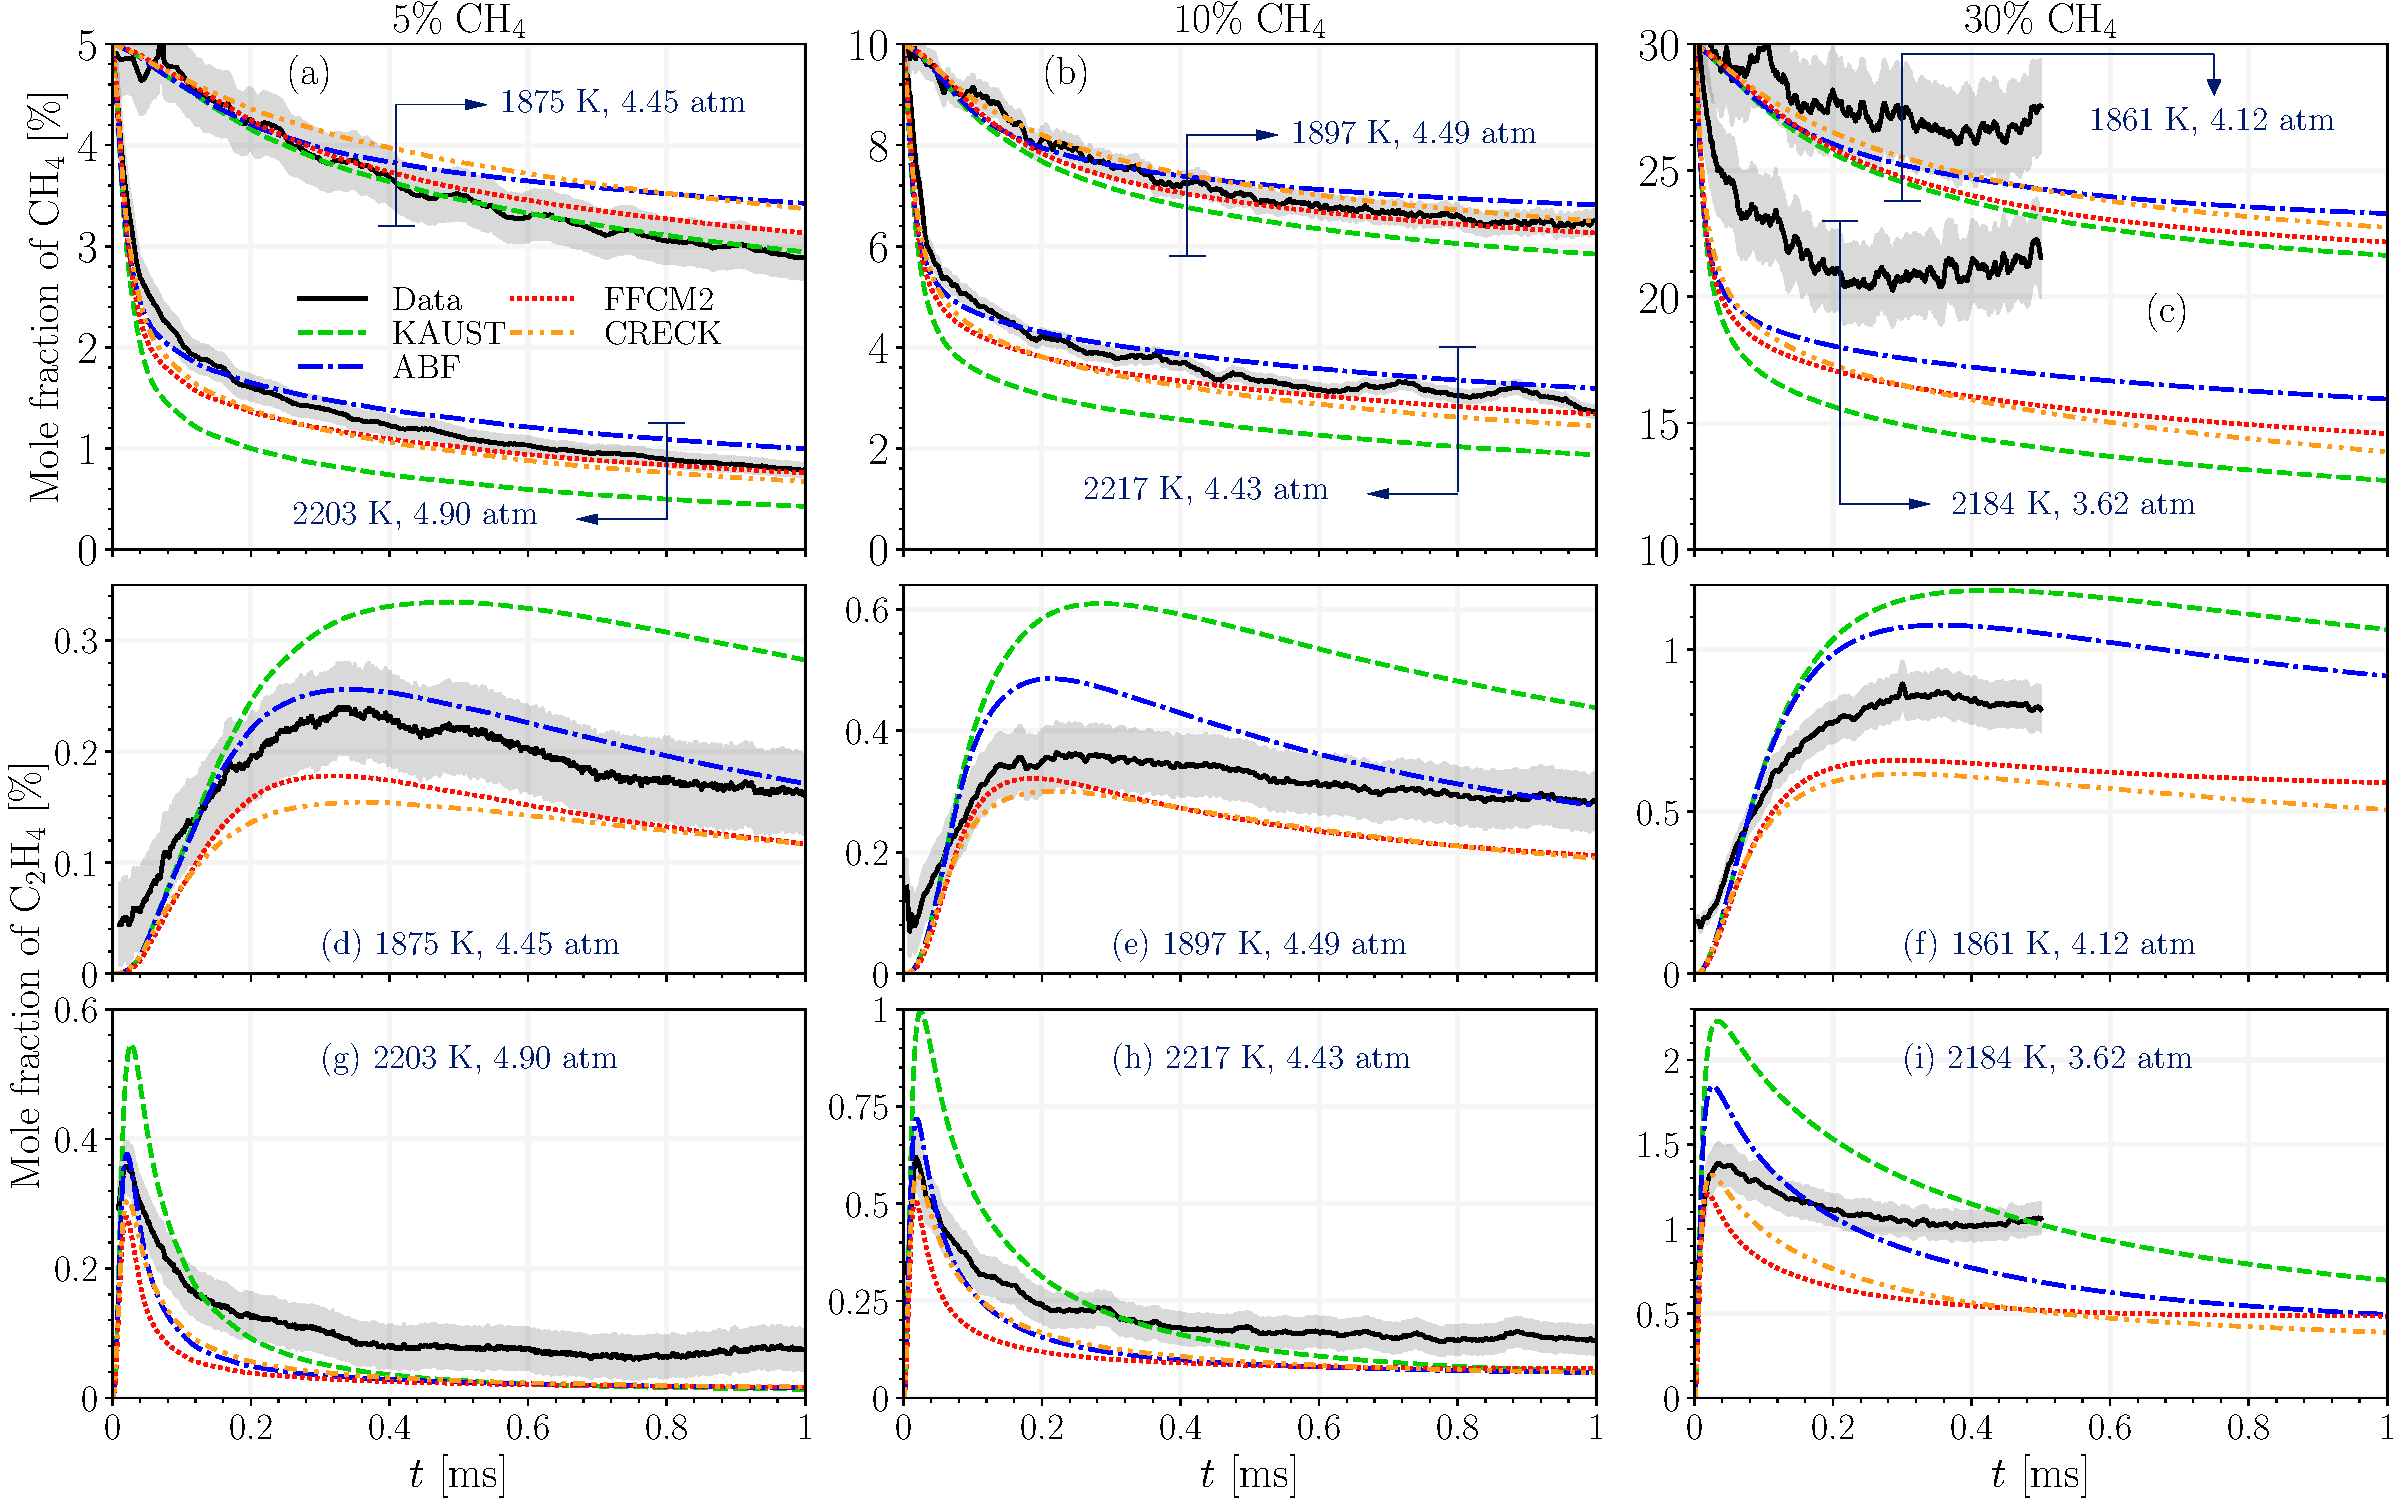
\includegraphics[width=1\textwidth]{Figures/Results/Paper2/CH4_C2H4_combined.pdf}
	\caption{The mole fraction time-history of (a-c) CH$_4$ and (d-i) C$_2$H$_4$ for 5\%, 10\%, and 30\% CH$_4$ pyrolysis for T$_5$$\approx$1900~K and 2200~K.}
	\label{fig:thx_ch4} 
\end{figure}


Methane conversion, defined as the fractional reduction in mole fraction, is $\approx$29\% for both 5\% and 10\% CH$_4$ at T$_5$$\approx$1900~K by 1~ms, but decreases from 78\% to 66\% at T$_5$$\approx$2200~K as fuel loading increases from 5\% to 10\%. These changes arise from variations in T$_5$, P$_5$, and coupled chemical–thermal effects. To isolate these effects, two additional sets of simulations were performed for 5\%, 10\%, and 30\% fuel loadings at T$_5$=1900~K and 2200~K and P$_5$=4.5~atm. These cases are referred to as ``Const-TP’’ and ``Const-P’’. In the Const-P simulations, a constant pressure of 4.5~atm was imposed instead of the measured pressure trace. In the Const-TP simulations, the temperature was also held constant at T$_5$ and the energy equation was not solved. Fig.~\ref{fig:ch4conversion_constTP_FFCM2} shows representative Const-TP and Const-P results using FFCM2, while the complete set of results is provided in Fig.~\ref{fig:ch4conversion_constTP}.

At T$_5$=1900~K, Const-TP simulations indicate that CH$_4$ conversion by 1~ms increases by approximately 2\% and 7\% at 10\% and 30\% loadings, respectively, relative to 5\% loading. Similar relative trends were observed for the other kinetic mechanisms. At T$_5$=2200~K, FFCM2 predicts full conversion ($>$99\%) by 1~ms, with the time to reach full conversion decreasing as fuel loading increases. In contrast, Const-P simulations show a much stronger reduction in CH$_4$ conversion with increasing fuel loading. At T$_5$=1900~K, the conversion at 1~ms decreases by nearly 20\% and 38\% for 10\% and 30\% loadings, respectively, compared to 5\% loading. These results indicate that the observed reduction in CH$_4$ conversion at higher fuel loadings is primarily driven by the endothermicity of pyrolysis, which causes faster and deeper temperature drops and consequently slows the decomposition reactions. The range of predicted temperature at 0.5~ms, T$_{\mathrm{(0.5\:ms)}}$, is compared for various loadings in Fig.~\ref{fig:temp_variation}, which demonstrates that T$_{\mathrm{(0.5\:ms)}}$ decreases with fuel loading. Moreover, the spread in the predicted temperature from kinetic mechanisms is $\approx$60~K for 30\% loading, larger than $\approx$47~K and $\approx$30~K for 10\% and 5\%, respectively.
\begin{figure}[!t]
	\centering
	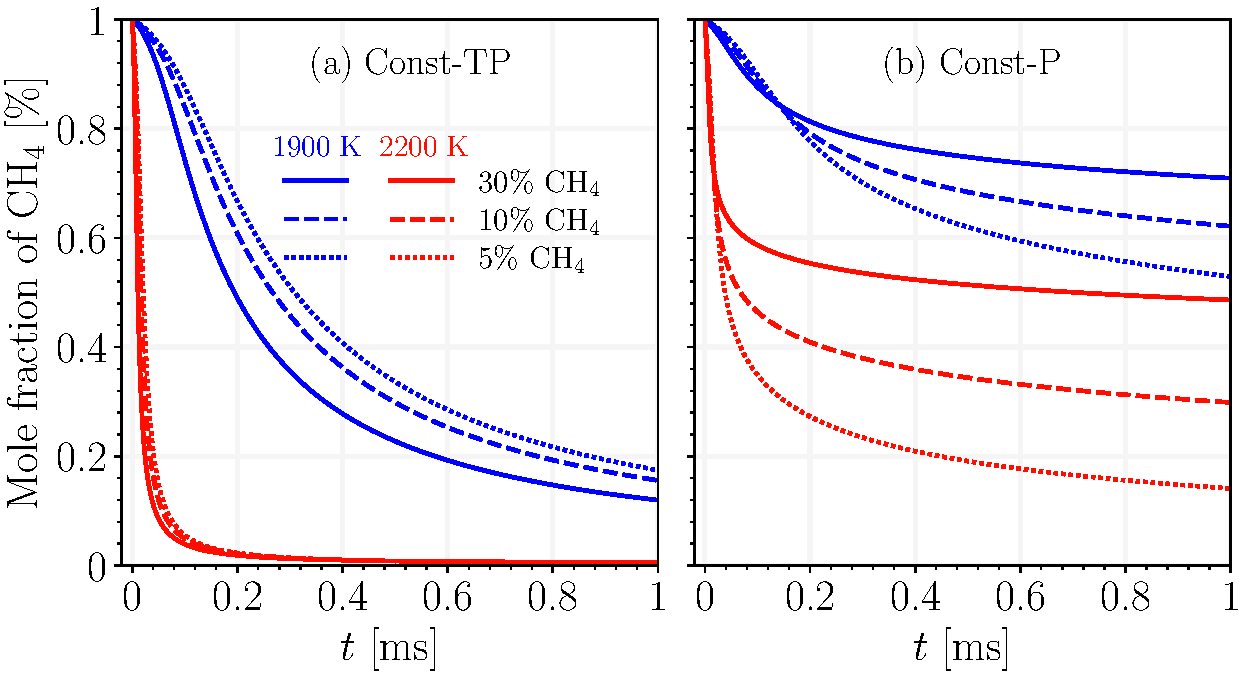
\includegraphics[width=0.75\textwidth]{Figures/Results/Paper2/CH4_conversion_constTP_FFCM2.pdf}
	\caption{The CH$_4$ conversion predicted using FFCM2 in (a) Const-TP and (b) Const-P simulations.}
	\label{fig:ch4conversion_constTP_FFCM2} 
\end{figure}

\begin{figure}[!t]
	\centering
	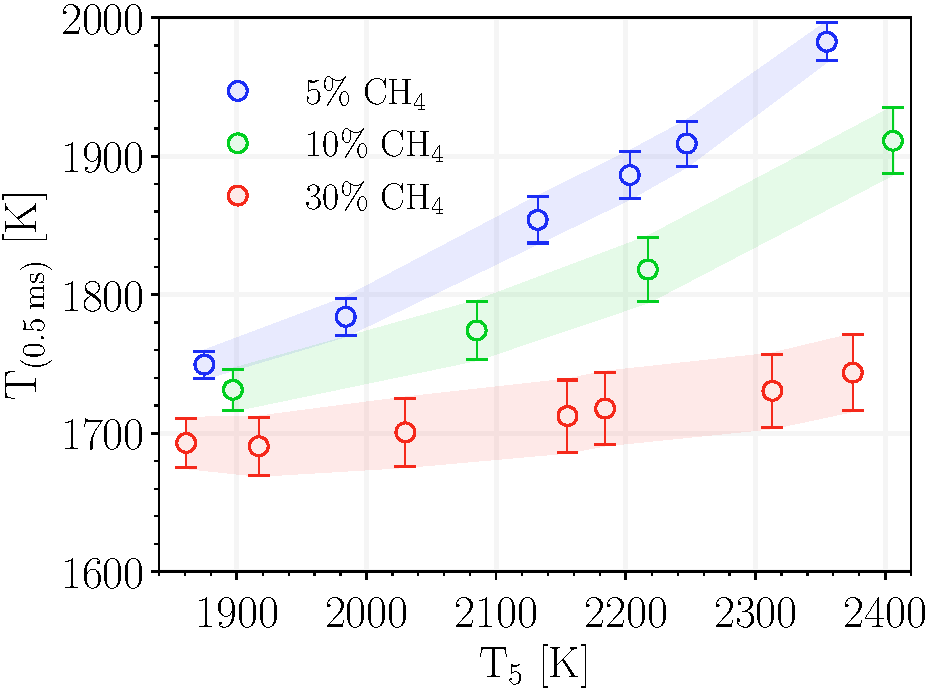
\includegraphics[width=0.55\textwidth]{Figures/Results/Paper2/temp_variation.pdf}
	\caption{
    Variation in predicted temperature at 0.5 ms for 5\%, 10\% and 30\% loadings over the studied T$_5$ range. Error bars and shaded regions represent the spread in predictions from four employed kinetic mechanisms.}
	\label{fig:temp_variation} 
\end{figure}


\begin{figure}[!t]
	\centering
	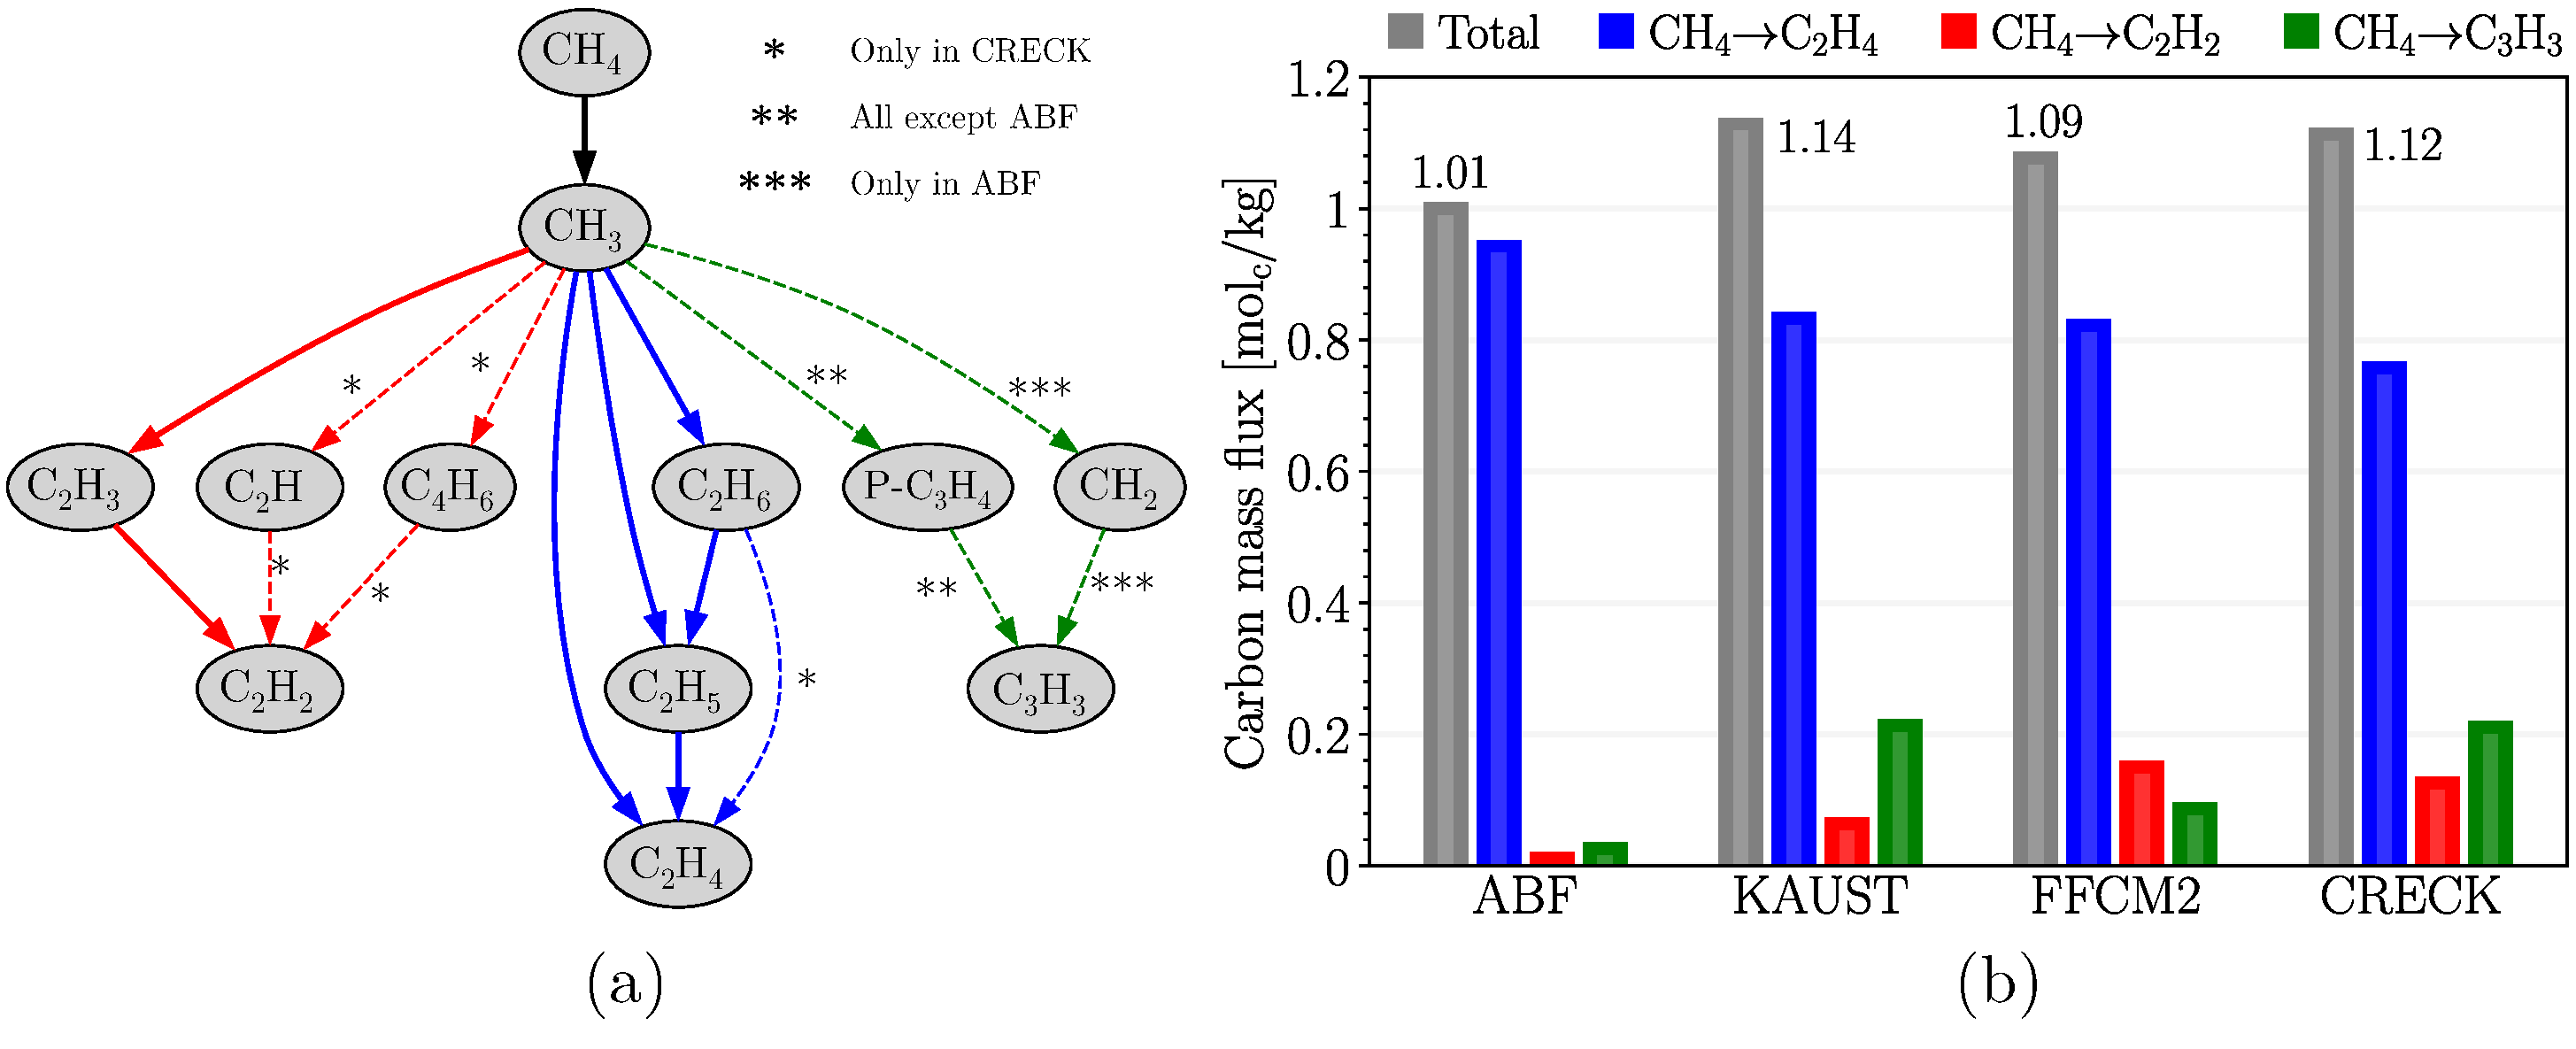
\includegraphics[width=1\textwidth]{Figures/Results/Paper2/CH4_pathways_barchart.pdf}
	\caption{(a) The common pathways for CH$_4$ conversion predicted using various kinetic mechanisms, and (b) the comparison of total flux from CH$_4$ to C$_2$H$_4$, C$_2$H$_2$, and C$_3$H$_3$ through exclusive pathways for 5\% loading at $\approx$2200~K.}
	\label{fig:ch4conversion_pathways} 
\end{figure}

As discussed previously, methane conversion is defined here as the fractional reduction in CH$_4$ mole fraction, normalized by its initial value, $1 - X_{\mathrm{CH_4}}/X_{\mathrm{CH_4,0}}$. This definition is widely used in shock-tube studies~\cite{agafonov2011shock, ferris2024experimental, panda2025understanding} to compute conversion from experimental measurements. However, it can deviate from the actual conversion defined based on the reduction in the carbon mass fraction of CH$_4$, $M_{\mathrm{c,CH_4}}/M_{\mathrm{c,CH_4,0}}$, because the total number of moles is not conserved during pyrolysis, whereas total carbon mass is conserved. Evaluation of all kinetic mechanisms shows that the mole-based definition systematically overpredicts methane conversion. The difference between mole- and mass-based conversion at 1~ms increases from an average of 1.1\% at 5\% loading to 5.8\% at 30\% loading. A comparison of conversion calculated using both definitions for all kinetic mechanisms is shown in Fig.~\ref{fig:ch4conversion_massmole}.



The comparison of predicted and measured CH$_4$ mole fraction (Fig.~\ref{fig:thx_ch4}a, b) indicates that among the kinetic mechanisms, FFCM2 provides the best agreement with the 5\% and 10\% data based on the root mean square error over 1~ms. At 30\% CH$_4$ (Fig.~\ref{fig:thx_ch4}c), all mechanisms overpredict conversion, with discrepancies increasing at higher $\mathrm{T_5}$. Additionally, the measured CH$_4$ mole fraction rises at 0.2~ms for T$_5$=1861~K and at 0.4~ms for T$_5$=2184~K, which is not observed in simulations. The apparent increase is likely caused by interference from overlapping C–H absorption bands of intermediate species formed more abundantly at high fuel loadings~\citep{ferris2024experimental}.





The ABF and KAUST mechanisms form the upper and lower bounds of the predicted CH$_4$ mole fraction across both conditions and the full $\mathrm{T_5}$ range. Methane conversion predicted by CRECK is comparable to ABF at $\mathrm{T_5}$$\approx$1900~K but increases with temperature, approaching FFCM2 predictions at $\mathrm{T_5}$$\approx$2200~K. Differences among mechanisms in the prediction of CH$_4$ conversion are not primarily due to variations in the rate constants of the dominant methane decomposition reactions, $\mathrm{CH_4+(M)\leftrightarrow CH_3+H}$ and $\mathrm{CH_4+H\leftrightarrow CH_3+H_2}$. A series of simulations were conducted using modified ABF, KAUST, and CRECK mechanisms, where the forward and reverse rate constants of both reactions were taken from FFCM2. As shown in Fig.~\ref{fig:temp_ch4_FFCM2}, the modification of dominant CH$_4$ decomposition reactions only alters temperature by $<$1\% and CH$_4$ mole fraction by $<$7\% over 1~ms of simulation.

Thus, modeling suggests the variation between the four kinetic mechanisms does not arise from the variability in the rate constants of methane decomposition reactions. Instead, we focus on the carbon flux through the reaction network and the carbon mass fraction (CMF) of species. The net progress rates of reactions were integrated to construct a directed graph~\citep{hagberg2008exploring}, where species are represented as nodes, and an edge connects species involved in a reaction. The direction of each edge indicates the net transfer of carbon from reactant to product, and its weight corresponds to the moles of carbon transferred along that reaction pathway over a given time interval, normalized by the total gas mass.

\begin{figure}[!t]
	\centering
	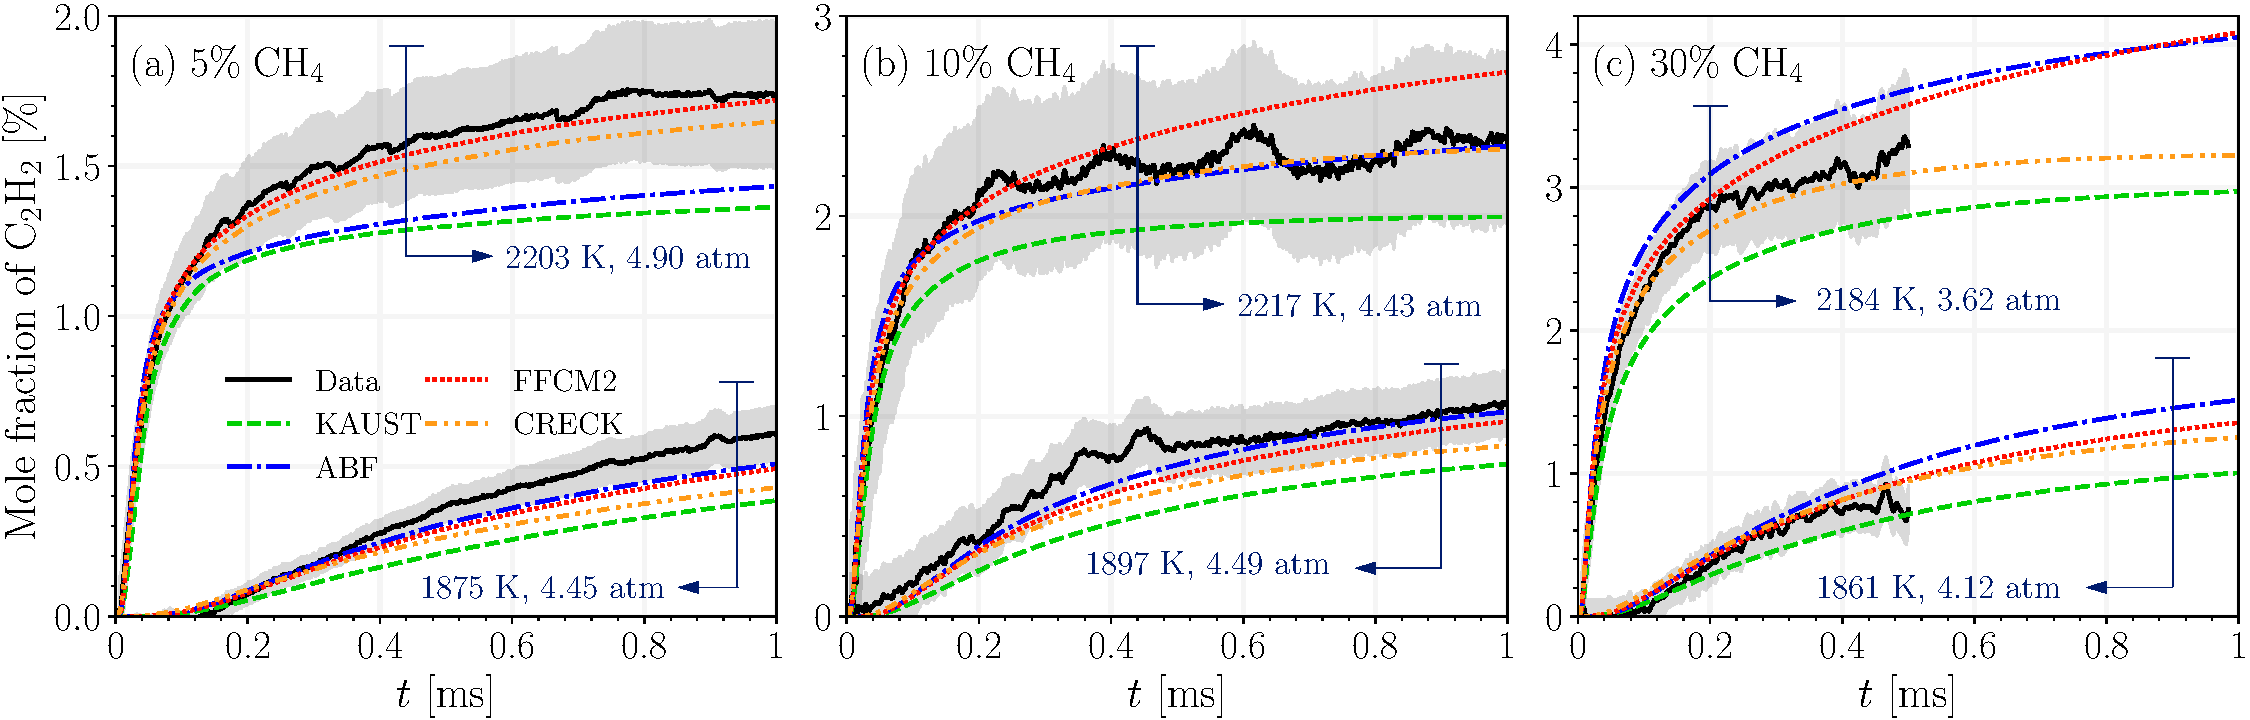
\includegraphics[width=1\textwidth]{Figures/Results/Paper2/C2H2_two_combined.pdf}
	\caption{The time history of C$_2$H$_2$ mole fraction for (a) 5\%, (b) 10\% and (c) 30\% CH$_4$ pyrolysis for T$_5$$\approx$1900~K and 2200~K}
	\label{fig:thx_c2h2} 
\end{figure}

\begin{figure}[!t]
	\centering
	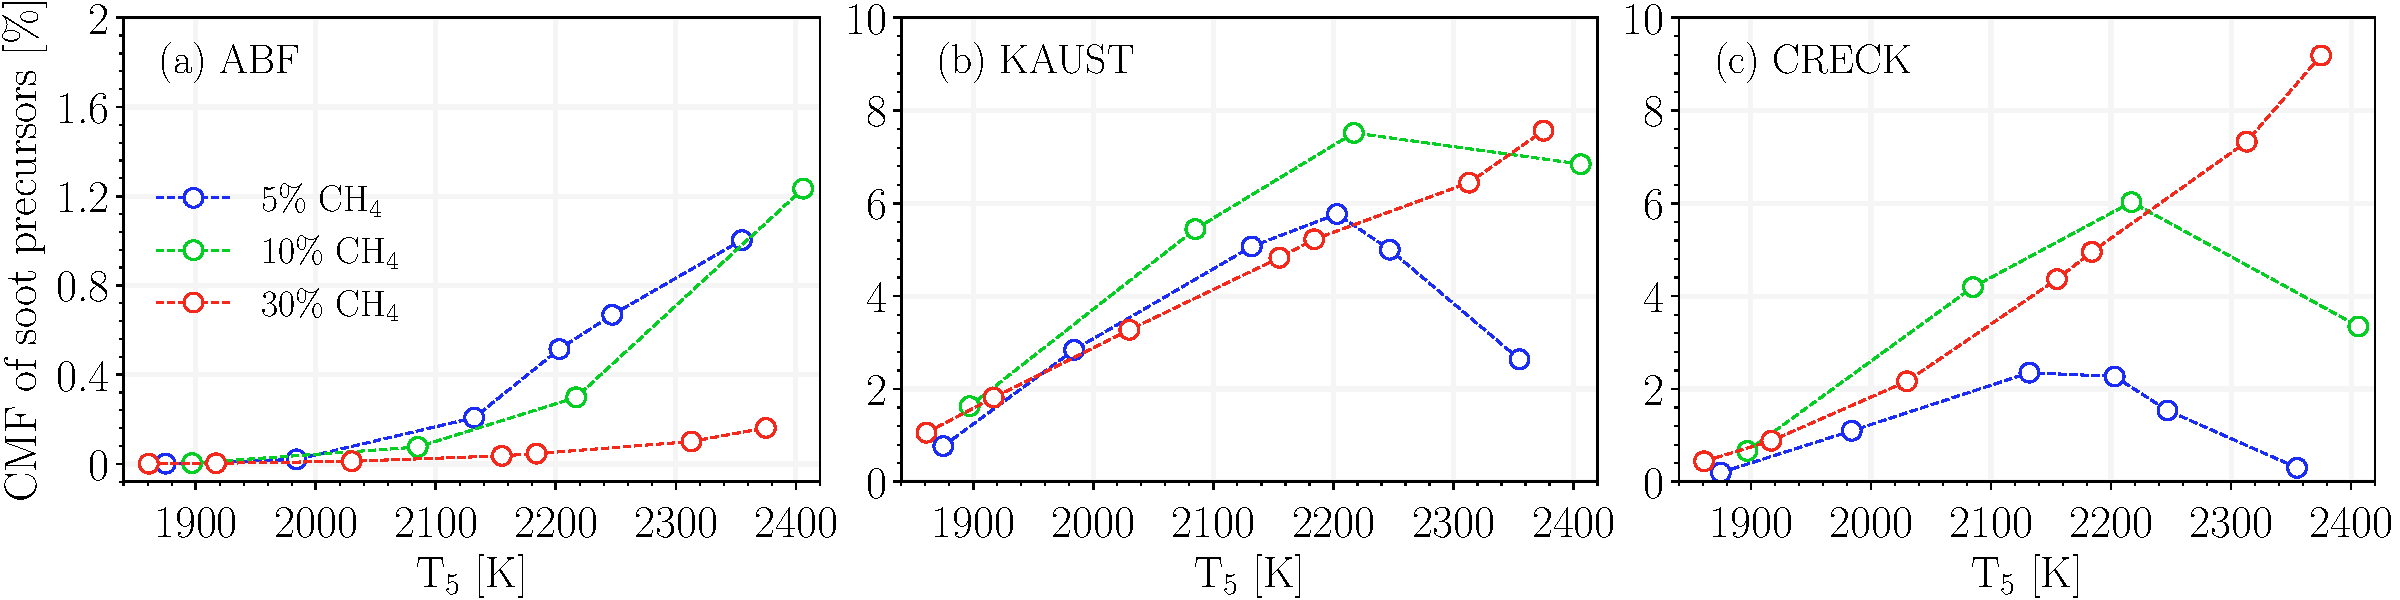
\includegraphics[width=1\textwidth]{Figures/Results/Paper2/cmf_spc.pdf}
	\caption{The CMF of soot precursors combined at 1~ms over the studied T$_5$ range predicted using (a) ABF, (b) KAUST, and (c) CRECK for 5\%, 10\%, and 30\% loadings.}
	\label{fig:spc_cmf} 
\end{figure}


The exclusive carbon pathways from CH$_4$ to C$_2$H$_2$, C$_2$H$_4$, and C$_3$H$_3$ were identified, and the corresponding carbon fluxes were compared for the kinetic mechanisms. Fig.~\ref{fig:ch4conversion_pathways}a illustrates major identified pathways of CH$_4$ consumption. Fig.\ref{fig:ch4conversion_pathways}b shows the representative results of carbon flux analysis for 5\% loading at 2200~K, suggesting that the persistent underprediction of CH$_4$ conversion by ABF is primarily due to lower carbon flux from CH$_4$ to C$_2$H$_2$ and C$_3$H$_3$ compared with the other mechanisms. While in ABF, C$_3$H$_3$ is predominantly produced via 
$\mathrm{C_2H_2+CH_2\leftrightarrow C_3H_3+H}$, in the other mechanisms propyne (P-C$_3$H$_4$) dehydrogenation ($\mathrm{P\text{-}C_3H_4\leftrightarrow C_3H_3+H}$) is responsible for C$_3$H$_3$ production. As shown in Fig.~\ref{fig:pc3h4_cmf}, CMF of P-C$_3$H$_4$ predicted by ABF remains below 0.03\% by 1~ms for all loadings and temperatures, which is nearly 60 times lower than the predictions of other kinetic mechanisms. Analysis of the reaction fluxes indicates that propyne (P–C$_3$H$_4$) is produced primarily via $\mathrm{C_2H_2 + CH_3 \leftrightarrow P\text{-}C_3H_4 + H}$. The forward rate constant of the reaction in ABF is nearly two orders of magnitude lower than the other mechanisms (Fig.~\ref{fig:pc3h4_reaction}), leading to underprediction of P-C$_3$H$_4$. FFCM2 predicts a larger CMF of P-C$_3$H$_4$ compared to KAUST and CRECK due to the lower subsequent consumption of C$_3$H$_3$ leading to carbon accumulation in P–C$_3$H$_4$.

The lower consumption of C$_3$H$_3$ in FFCM2 is due to the lack of propargyl recombination reaction, 2C$_3$H$_3$ $\leftrightarrow$ A1, which is dominant in ABF and KAUST, and a major consumption reaction in CRECK. On other hand,  C$_3$H$_3$+CH$_3$$\leftrightarrow$C$_4$H$_6$ is the dominant C$_3$H$_3$ consumption reaction in CRECK and FFCM2. The peak CMF of C$_3$H$_3$ consistently decreases in all kinetic mechanisms is primarily due to lower CH$_4$ conversion at higher loadings. KAUST exhibits the highest carbon flux from C$_3$H$_3$ to A1, which rapidly propagates to larger PAHs. At 5\% and 10\% loadings, nearly 23\% of the total carbon mass resides in $\mathrm{C_6}$ and larger species ($\mathrm{C_{\ge6}}$) in KAUST, whereas the CMF of $\mathrm{C_{\ge6}}$ remains below 12\% for CRECK and ABF.



More than 55\% of the carbon flux from CH$_4$ is directed to C$_2$H$_4$ across all mechanisms and conditions through two dominant pathways: $\mathrm{CH_4}\rightarrow\mathrm{CH_3}\rightarrow\mathrm{C_2H_5}\rightarrow\mathrm{C_2H_4}$ and $\mathrm{CH_4}\rightarrow\mathrm{CH_3}\rightarrow\mathrm{C_2H_6}\rightarrow\mathrm{C_2H_5}\rightarrow\mathrm{C_2H_4}$.
As shown in Fig.~\ref{fig:thx_ch4}d-i, ABF and KAUST overpredict the C$_2$H$_4$ peak at 10\% and 30\% loadings. FFCM2 and CRECK yield similar C$_2$H$_4$ profiles and reproduce the peak more accurately. The subsequent decline in C$_2$H$_4$ results from carbon transfer to C$_2$H$_2$ through the dominant pathway $\mathrm{C_2H_4}\rightarrow\mathrm{C_2H_3}\rightarrow\mathrm{C_2H_2}$ except for CRECK, which includes an additional direct pathway from C$_2$H$_4$ to C$_2$H$_2$ via the third-body reaction $\mathrm{C_2H_4} + \mathrm{M}\leftrightarrow \mathrm{C_2H_2} + \mathrm{H_2} + \mathrm{M}$.




Time-resolved mole fraction of C$_2$H$_2$ is shown in Fig.~\ref{fig:thx_c2h2}. At 30\% loading, C$_2$H$_2$ measurements are better captured by the kinetic mechanisms compared to CH$_4$ because the selected transitions near 2998~nm targeting the asymmetric C-H stretch of acetylene are spectrally isolated from other hydrocarbons~\citep{jeevaretanam2023transient}.
At 5\% loading, a noticeable drop is observed in ABF's prediction of C$_2$H$_2$ relative to the other mechanisms from 1875~K to 2203~K due to the rapid accumulation of carbon in A1. The CMF of $\mathrm{C_{\ge6}}$ changes from 0.7\% to 10.7\% for ABF and from 3.3\% to 6\% for CRECK. FFCM2 best captures C$_2$H$_2$ yield at 5\% over the entire T$_5$ range. At 10\% loading and 2217~K, all model predictions fall within the measurement uncertainty, but their trends differ slightly. FFCM2 predicts a faster rise after 0.4~ms in C$_2$H$_2$ compared to ABF and CRECK, which better reproduce the trends in the measurements. 
At 30\% loading, ABF and KAUST closely predict the upper and lower uncertainty range of C$_2$H$_2$ mole fraction at both temperatures, respectively. The high C$_2$H$_2$ predictions by ABF, despite its low CH$_4$ conversion values, are the compound effect of having the highest carbon flux from C$_2$H$_4$ to C$_2$H$_2$ and the lowest carbon flux from C$_2$H$_2$ to C$_3$H$_3$.

Fig.~\ref{fig:spc_cmf} shows the dependence of the carbon mass fraction (CMF) of soot precursors on T$_5$ and fuel loading at 1~ms. Results for FFCM2 are not included because it does not contain PAH chemistry. ABF predicts the lowest CMF ($\le$1.2\%) among the kinetic mechanisms, with a monotonic increase with T$_5$ and a decrease with fuel loading. In contrast, KAUST and CRECK exhibit a bell-shaped temperature dependence at 5\% and 10\% loadings, while the CMF increases monotonically with T$_5$ at 30\% loading. 


These trends arise from the combined effects of endothermic cooling during pyrolysis and the intrinsic temperature dependence of precursor formation in each kinetic mechanism. The Const-TP results (Fig.~\ref{fig:cmf_spc_constTP}) show that all mechanisms predict a bell-shaped CMF profile with temperature. The peak CMF occurs near 2075~K for ABF, but around 1875~K for KAUST and CRECK. As shown in Fig.~\ref{fig:temp_variation}, the predicted gas temperature at 0.5~ms never exceeds 2075~K under the studied conditions, so all ABF cases remain on the rising side of the bell-shaped curve, yielding a persistently increasing trend with T$_5$. For KAUST and CRECK, the predicted temperature exceeds 1875~K at 5\% and 10\% loadings when T$_5$$>$ 2200~K, causing the CMF of soot precursors to decrease beyond this point. At 30\% loading, stronger endothermic cooling limits the temperature rise, preventing the system from reaching the descending branch of the bell-shaped curve and resulting in a monotonic increase in CMF with T$_5$.

